\documentclass[conference]{IEEEtran}

\usepackage[T1]{fontenc}
\usepackage{cite}
\usepackage{amsmath,amssymb,amsfonts}
\usepackage{algorithmic}
\usepackage{graphicx}
\usepackage{textcomp}
\usepackage{xcolor}
\usepackage{booktabs}
\usepackage{multirow}
\usepackage[hyphens]{url}
\Urlmuskip=0mu plus 2mu\relax
\usepackage{balance}
\usepackage{microtype}

\sloppy
\emergencystretch=3em

\def\BibTeX{{\rm B\kern-.05em{\sc i\kern-.025em b}\kern-.08em
    T\kern-.1667em\lower.7ex\hbox{E}\kern-.125emX}}

\begin{document}

\title{SCHR-Bench: Evaluating Security-Critical Hallucinations in LLM-Assisted Binary Reverse Engineering via Ground-Truth Mutations}

\author{
\IEEEauthorblockN{
Tan-Phat Nguyen\IEEEauthorrefmark{1},
Thien-Nhan Do\IEEEauthorrefmark{1},
Trong-Duy Nguyen\IEEEauthorrefmark{1},
Hong-Phuc Vo\IEEEauthorrefmark{1}, and
Mai-Hoang Dinh\IEEEauthorrefmark{1}\IEEEauthorrefmark{2}
}
\IEEEauthorblockA{\IEEEauthorrefmark{1}Department of Information Assurance, FPT University, Ho Chi Minh City, Vietnam}
\IEEEauthorblockA{Email: \{phatntse173285, nhandtse194134, duyntse194413, phuchvse203844\}@fpt.edu.vn}
\IEEEauthorblockA{\IEEEauthorrefmark{2}Corresponding Author: dinhmh@fe.edu.vn}
}

\maketitle

\begin{abstract}
Large Language Models (LLMs) are increasingly integrated into software reverse engineering (SRE) pipelines to interpret decompiled pseudocode, synthesize functional intent, and accelerate incident response. However, in security-critical operations such as malware triage and vulnerability auditing, LLM hallucinations can yield severe operational failures by inverting control-flow predicates, misidentifying encryption constants, or overlooking stealthy evasion logic. Existing code evaluation benchmarks primarily measure surface syntactic fluency (e.g., BLEU-4) or syntactic re-compilability, which fail to capture subtle yet critical semantic inversions. To bridge this gap, we introduce \textbf{SCHR-Bench}, an automated benchmarking framework designed to quantify \textbf{Security-Critical Hallucination Rates (SCHR)} using differential binary mutations backed by deterministic ground truth. We construct 40 controlled C security-logic function pairs (80 stripped x86-64 PE binaries) spanning five security decision archetypes: Mock Debugger Policy (Category A), Toy Byte Decoder (Category S), Persistence State Mock (Category P), Environment Signal Mock (Category E), and Control-Flow \& Boundary Logic (Category C). Each mutation is dynamically verified via Experiment E0 across 80 targeted test vectors (160 execution assertions) to confirm 100\% non-neutral behavioral divergence. Across 540 deterministic evaluation runs ($\tau = 0.0, \text{seed} = 42$), we benchmark general-purpose (\texttt{LLaMA-3.1 8B}) and code-specialized (\texttt{Qwen2.5-Coder 14B}) open-weight models across three context escalation tiers (CT1--CT3, $N=80$ per tier) and four Obfuscator-LLVM (OLLVM) transformation configurations (Obf0--Obf3, $N=10$ stratified subsample), while specifying CT4 as an interprocedural architectural blueprint. Our empirical findings demonstrate that: (1) high pairwise lexical overlap between explanations of original and mutated binaries ($\text{BLEU-4} \in [0.358, 0.462]$) routinely obscures severe security hallucinations, with \texttt{LLaMA-3.1 8B} exhibiting a baseline CT1 SCHR of 38.8\% [95\% Wilson CI: 28.8\%, 49.7\%] and a Mutant Miss Rate of 32.5\%; (2) code-specialized pretraining in \texttt{Qwen2.5-Coder 14B} reduces baseline CT1 SCHR to 23.8\% [15.8\%, 34.1\%] and CT3 SCHR to 18.8\% [11.7\%, 28.7\%], though bitwise decryption loops (Category S) remain a persistent bottleneck (56.2\% SCHR for both models); (3) appending x86-64 disassembly and API metadata (CT2/CT3) yields directional error reductions ($38.8\% \rightarrow 35.0\%$ for LLaMA-3.1; $23.8\% \rightarrow 18.8\%$ for Qwen2.5-Coder), though McNemar's paired test ($p \in [0.289, 0.752]$) indicates that passive context concatenation does not fully overcome pseudocode primacy; and (4) combined OLLVM obfuscation (\path{Obf3_Combined}) elevates SCHR from 30.0\% to 40.0\% on LLaMA-3.1 and doubles it from 10.0\% to 20.0\% on Qwen2.5-Coder. Finally, we contextualize our findings with a static forensic triage case study on a VMProtect-packed Gh0stRAT PE32 sample.
\end{abstract}

\begin{IEEEkeywords}
Binary Reverse Engineering, Large Language Models, Hallucination Benchmarking, Software Security, Differential Mutation Testing, Malware Triage, Code Obfuscation.
\end{IEEEkeywords}

\section{Introduction}
Software Reverse Engineering (SRE) of compiled, stripped machine code is fundamental to modern cybersecurity operations, including malware triage, threat intelligence extraction, firmware vulnerability discovery, and incident containment. Because raw x86-64 assembly instructions impose substantial cognitive burdens on human analysts, modern reverse engineering workflows depend heavily on decompilation frameworks like Ghidra~\cite{ghidra2024nsa} and IDA Pro to reconstruct high-level C-like pseudocode. Recently, Large Language Models (LLMs) have emerged as copilot assistants capable of summarizing decompiled subroutines, identifying programmatic intent, and reconstructing stripped symbol names~\cite{sun2024llm4decompile,hui2024qwen25coder,dubey2024llama3}.

\begin{figure*}[t]
\centering
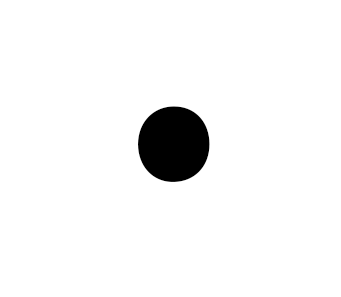
\includegraphics[width=0.94\textwidth]{figures/fig1.png}
\caption{Decoupled Multi-Tier Testbed Architecture of SCHR-Bench: (1) Tier 1 GPU Host dedicated to deterministic local LLM inference ($\tau = 0.0, \text{seed} = 42$); (2) Tier 2 Kali Linux headless automation orchestrating MinGW-w64 cross-compilation, OLLVM obfuscation, Ghidra decompilation, and E0 ground-truth verification; and (3) Tier 3 isolated Windows 11 environment dedicated to offline static forensic inspection and PE header triage using DIE and PE-bear with zero runtime malware execution.}
\label{fig:architecture}
\end{figure*}

Despite these capabilities, LLMs exhibit a pervasive failure mode: \textit{hallucination}~\cite{ji2023hallucination}. While hallucinating benign syntax in standard software development causes immediate compiler errors, hallucinations during security analysis carry severe operational consequences. A model that inverts an anti-debugging policy check, miscomputes an XOR decryption key, or misjudges a persistence state transition can lead incident responders to misclassify active threats or overlook critical logic flaws. As demonstrated by Basque et al.~\cite{basque2025synergy}, while LLMs accelerate initial comprehension for novice analysts, misleading explanations impose heavy verification overhead, forcing human defenders into manual debugging to validate deceptive outputs.

Evaluating LLM hallucinations in binary reverse engineering presents two major challenges:
\begin{enumerate}
    \item \textbf{Absence of Deterministic Behavioral Ground Truth:} Decompiled pseudocode is inherently lossy and discards variable names, types, and comments. Prior frameworks such as VeRA~\cite{alrabaee2022vera} rely on debug symbol tables to evaluate variable name and type recovery, remaining blind to whether the model comprehends underlying security control-flow invariants.
    \item \textbf{Inadequacy of Surface Lexical Metrics:} Classical NLP metrics like BLEU-4~\cite{papineni2002bleu} reward surface lexical overlap while remaining blind to critical logical inversions. An explanation generated for a mutated binary can share high lexical overlap with the original binary's explanation while completely inverting a conditional branch (\texttt{JZ} vs.\ \texttt{JNZ}). Similarly, syntactic re-compilability (as in Decompile-Eval~\cite{decompileeval2024}) only confirms grammatical syntax, offering no guarantee that security-critical semantics are preserved.
\end{enumerate}

To overcome these challenges, this paper presents \textbf{SCHR-Bench}, an automated benchmarking framework utilizing differential binary mutations with strictly verifiable ground truth. By pairing original C security-logic functions ($f_{\text{orig}}$) with semantically divergent, minimally mutated counterparts ($f_{\text{mut}}$), compiling them into stripped x86-64 PE binaries, and verifying behavioral non-neutrality dynamically via automated test vectors (Experiment E0), SCHR-Bench establishes an unambiguous oracle for measuring security-critical hallucinations. Our complete dataset, extraction scripts, and 540 raw evaluation logs are publicly available at \url{https://github.com/phat1310/IAM302t_SCHR_Bench}.

\section{Related Work and Research Motivation}

\subsection{Decompilation Challenges in Security Audits}
Static decompilation frameworks lift raw machine instructions into control-flow graphs (CFGs) and structured Abstract Syntax Trees (ASTs)~\cite{yakdan2015norepdb}. However, compiler optimizations (\texttt{-O2}), register reuse, and control-flow obfuscation often cause decompilers to emit synthesized temporaries (\path{uVar1}, \path{param_1}), ambiguous pointer casts, and convoluted branch conditions~\cite{schwarz2002disassembly,cifuentes1995decompilation}. When analyzing stripped binaries, these decompilation artifacts frequently induce speculative misinterpretations by LLMs.

\subsection{LLMs in Binary Reverse Engineering and Distinct Positioning}
Recent efforts such as LLM4Decompile~\cite{sun2024llm4decompile} pretrain neural models to reconstruct source code directly from assembly, while complementary studies leverage foundation models (\texttt{LLaMA-3}~\cite{dubey2024llama3}, \texttt{Qwen2.5-Coder}~\cite{hui2024qwen25coder}) to summarize decompiled subroutines. Existing benchmarks such as VeRA~\cite{alrabaee2022vera}, Decompile-Eval~\cite{decompileeval2024}, and RevLLM~\cite{revllm2024} evaluate symbol recovery, general algorithmic syntax pass rates, or subjective intent tags. In contrast, SCHR-Bench is specifically designed to quantify \textbf{security-critical semantic inversions} across stripped binaries and OLLVM obfuscation transformations using an execution-verified mutation oracle.

\section{The SCHR-Bench Framework}

\subsection{Problem Formulation and Metric Definitions}
Let $B_{\text{orig}}$ and $B_{\text{mut}}$ represent a pair of stripped binary executables compiled from source functions $f_{\text{orig}}$ and $f_{\text{mut}}$, respectively, where $f_{\text{mut}} = \mathcal{M}(f_{\text{orig}})$ under a formal mutation operator $\mathcal{M}$. The decompiler extracts context representation $\mathcal{D}_k(B)$ at context tier $k \in \{\text{CT1, CT2, CT3}\}$. When prompted with $\mathcal{D}_k(B)$ and a targeted semantic query $Q$, an LLM generates a structured prediction $\hat{y}_i$ and natural language explanation $\mathcal{Y}_i$.

To rigorously evaluate model reliability across all $N=80$ binaries ($40$ original and $40$ mutated executables), we formulate two primary metrics:
\begin{enumerate}
    \item \textbf{Security-Critical Hallucination Rate (SCHR):} Measures the proportion of evaluation instances ($N=80$) in which the LLM predicts an incorrect security decision outcome ($\hat{y}_i \neq y_i^*$) relative to the execution-verified ground truth $y_i^*$:
    \begin{equation}
    \text{SCHR} = \frac{1}{N} \sum_{i=1}^N \mathbb{I}\left( \hat{y}_i \neq y_i^* \right)
    \end{equation}
    where $\mathbb{I}(\cdot)$ is the indicator function.
    \item \textbf{Mutant Miss Rate:} Measures the proportion of mutated binaries ($N_{\text{mut}} = 40$) on which the LLM fails to capture the mutated security semantics:
    \begin{equation}
    \text{Miss Rate} = \frac{1}{N_{\text{mut}}} \sum_{j=1}^{N_{\text{mut}}} \mathbb{I}\left( \hat{y}_{\text{mut}, j} \neq y_{\text{mut}, j}^* \right)
    \end{equation}
\end{enumerate}

We compute 95\% confidence intervals using the Wilson score interval~\cite{wilson1927probable}:
\begin{equation}
w = \frac{\hat{p} + \frac{z^2}{2N} \pm z \sqrt{\frac{\hat{p}(1-\hat{p})}{N} + \frac{z^2}{4N^2}}}{1 + \frac{z^2}{N}}
\end{equation}
where $\hat{p}$ is the sample error proportion and $z = 1.96$. Because CT1, CT2, and CT3 are evaluated on the exact same 80 binaries, we test paired differences using McNemar's test~\cite{mcnemar1947note} with continuity correction: $\chi^2 = \frac{(|b - c| - 1)^2}{b + c}$, where $b$ counts instances where CT1 erred and CT2/CT3 succeeded, and $c$ counts instances where CT1 succeeded but CT2/CT3 erred.

\subsection{Ground-Truth Evaluation Protocol and Pairwise BLEU-4}
To eliminate subjective grading bias in our quantitative tables, SCHR-Bench implements a deterministic evaluation pipeline (\path{step3_mcp_server_and_benchmark.py} and \path{step4_compute_statistics_and_tables.py}):
\begin{enumerate}
    \item \textbf{Deterministic Behavioral Oracle Verification:} For each binary $B_i$, the model is queried at $\tau = 0.0, \text{seed} = 42$ with $\mathcal{D}_k(B_i)$ and the function pair's discriminating input condition from \path{ground_truth_manifest.json}, returning a structured JSON object containing \path{predicted_return} ($\hat{y}_i \in \{0, 1\}$) and a single-sentence \texttt{explanation} ($\mathcal{Y}_i$). Additionally, our repository includes a 150-item multiple-choice suite (\path{dataset/gold_set_mcq.json}) with balanced option keys (A=31, B=37, C=41, D=41).
    \item \textbf{Pairwise Explanation Similarity (Orig vs.\ Mut BLEU-4):} To evaluate whether surface lexical overlap can distinguish between an original function $f_{\text{orig}}$ and its mutant $f_{\text{mut}}$, we compute the corpus-level BLEU-4~\cite{papineni2002bleu} between the LLM's explanation $\mathcal{Y}_{\text{orig}}$ and $\mathcal{Y}_{\text{mut}}$ across all 40 pairs.
\end{enumerate}

\begin{figure*}[t]
\centering
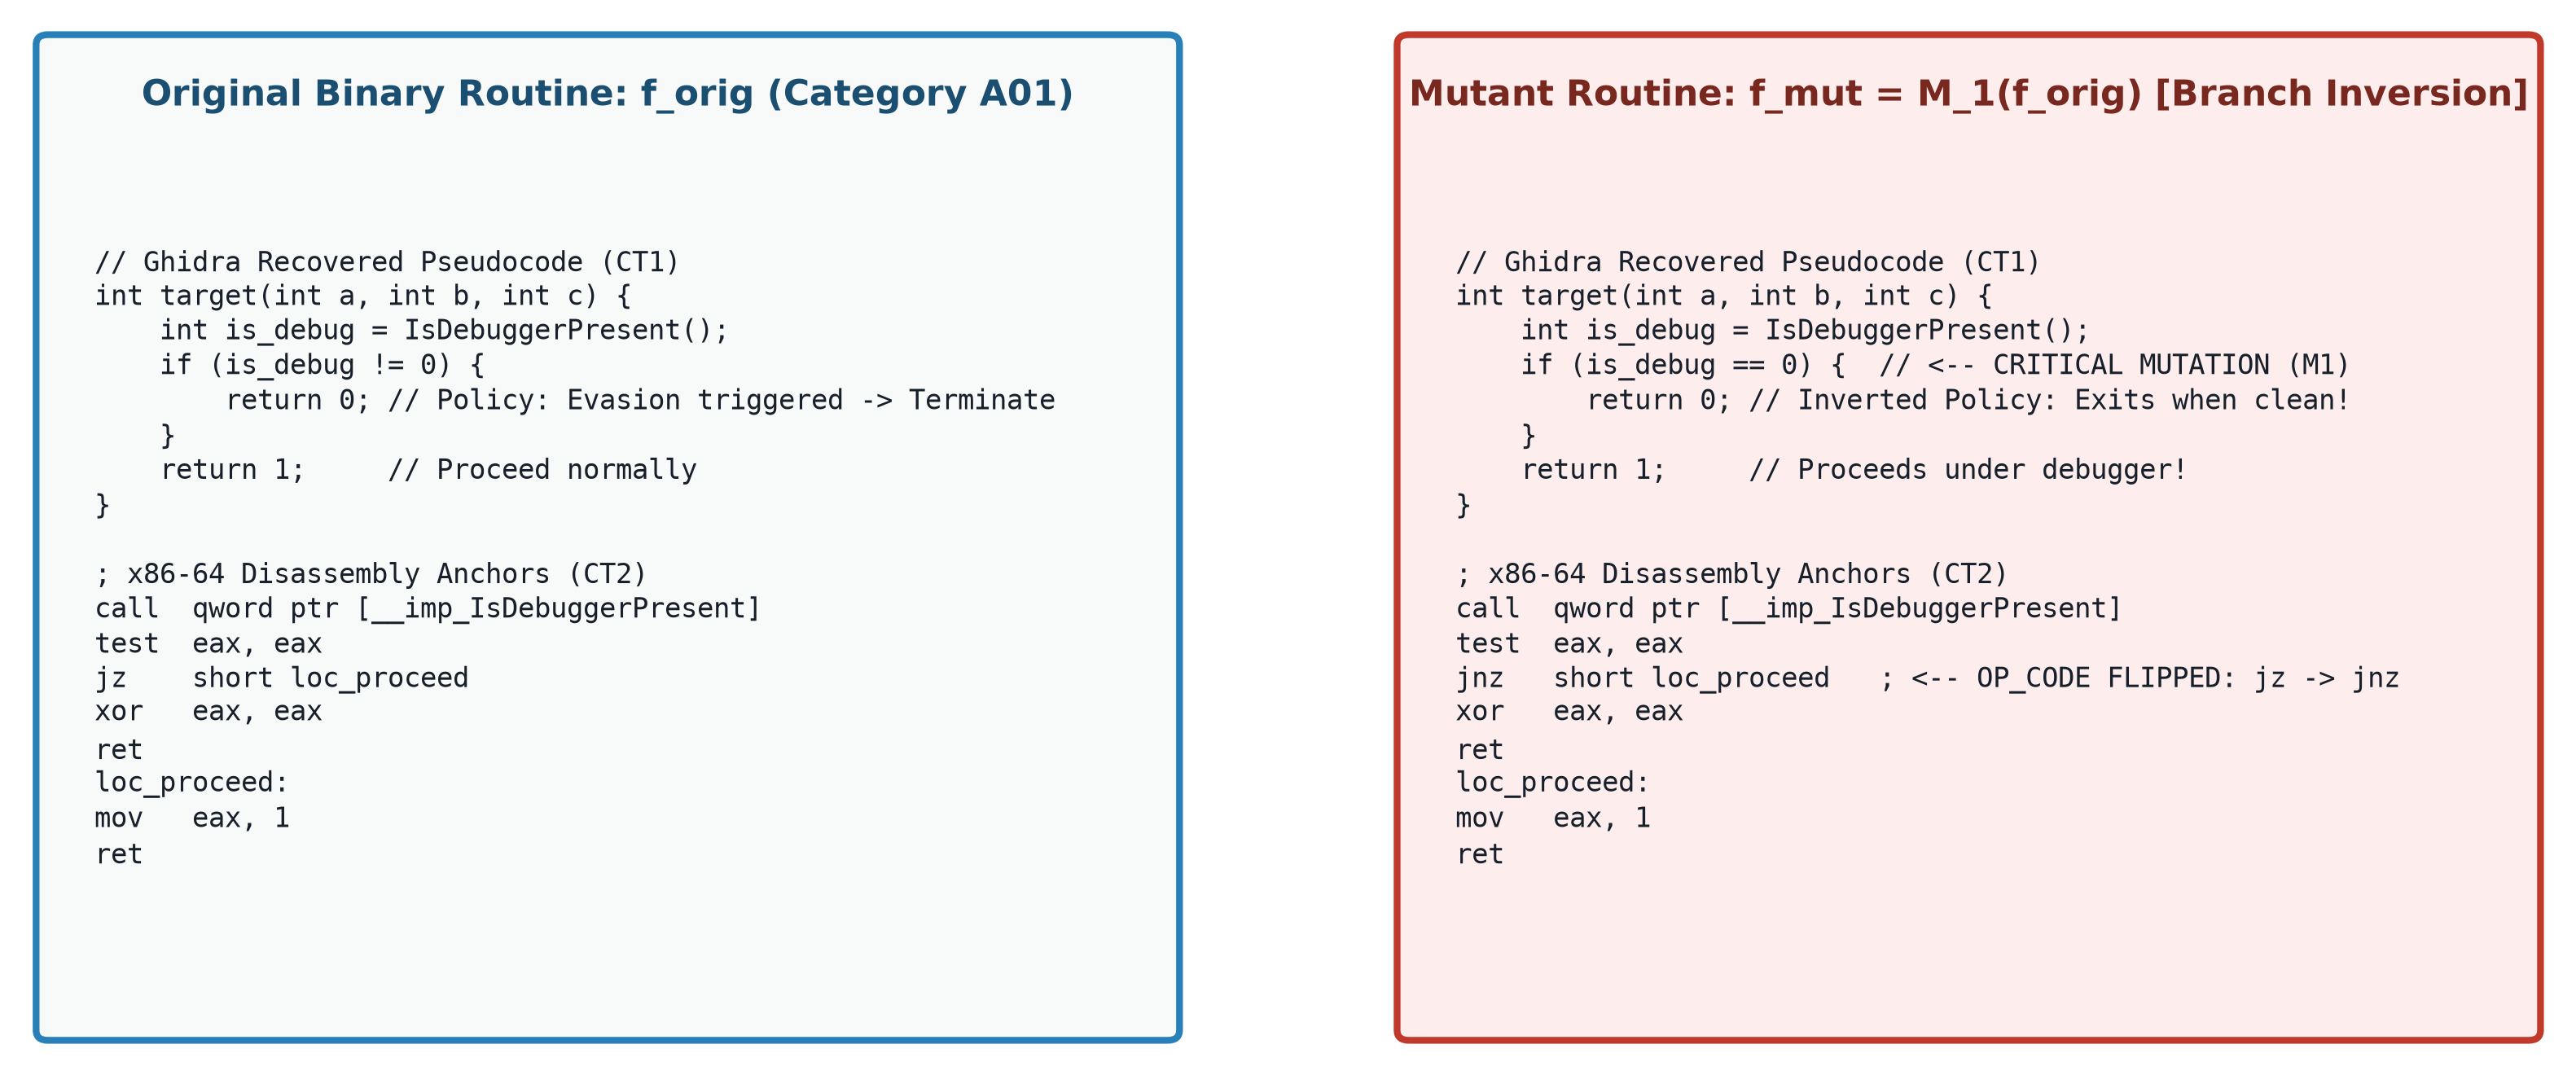
\includegraphics[width=0.92\textwidth]{figures/fig2_decompilation_diff.png}
\caption{Visualizing the Semantic Inversion Gap: (Left) Decompiled Ghidra C pseudocode of original versus mutated routines (human annotations are added solely for expository clarity; prompts fed to LLMs contain stripped pseudocode with zero comments); (Right) Corresponding ground-truth x86-64 disassembly diff showing branch condition inversion (\texttt{JZ} vs.\ \texttt{JNZ}).}
\label{fig:decompilation_diff}
\end{figure*}

\subsection{Controlled Security-Logic Kernels and Compilation Pipeline}
To isolate core control-flow and data-flow invariants from operating system non-determinism while ensuring 100\% execution safety, all 40 function pairs (80 C files in \path{dataset/SCHR_Bench_C_Functions/src/}) are authored as self-contained, deterministic C security-logic kernels with a uniform signature \texttt{int target(int a, int b, int c)} (pure local logic with no OS modifications). Each pair models a canonical security decision archetype across five balanced categories (8 pairs / 16 binaries per category):
\begin{itemize}
    \item \textbf{Category A (Mock Debugger Policy --- \texttt{A01}--\texttt{A08}):} Models anti-debugging decision policies including debugger flag checks, bitmask inspections, timing delta thresholds, hardware breakpoint counts, and parent-process token verification.
    \item \textbf{Category S (Toy Byte Decoder --- \texttt{S01}--\texttt{S08}):} Models payload decoding routines including single-byte XOR masks, rolling key schedules, additive/subtractive shifts, bitwise nibble rotations, and checksum verification loops.
    \item \textbf{Category P (Persistence State Mock --- \texttt{P01}--\texttt{P08}):} Models persistence state-machine transitions comparing privilege flags, target hive selectors, retry counters, and fallback installation paths.
    \item \textbf{Category E (Environment Signal Mock --- \texttt{E01}--\texttt{E08}):} Models sandbox and VM evasion predicates evaluating RAM size thresholds, CPU core counts, MAC prefix identifiers, and uptime windows.
    \item \textbf{Category C (Control-Flow \& Boundary Logic --- \texttt{C01}--\texttt{C08}):} Models multi-stage authentication guards, state-machine dispatchers, compound boolean predicates, and buffer boundary checks.
\end{itemize}

All 80 C files are cross-compiled on Tier 2 using MinGW-w64 (\path{x86_64-w64-mingw32-gcc} with flags \texttt{-O2 -s}) into stripped 64-bit Windows PE executables. Stripping removes all symbol tables and function names, ensuring models reason strictly over decompiled ASTs and assembly instructions. For adversarial obfuscation evaluation (Section~\ref{sec:rq4}), functions are transformed under four levels in \path{results/decompiled_contexts_80.json}: \texttt{Obf0} (unobfuscated \texttt{-O2 -s} baseline), \path{Obf1_CFF} (\texttt{-mllvm -fla}, Control-Flow Flattening), \path{Obf2_Sub} (\texttt{-mllvm -sub}, Instruction Substitution), and \path{Obf3_Combined} (\texttt{-mllvm -fla -mllvm -sub -mllvm -bcf}, Combined Flattening, Substitution, and Bogus Control Flow).

\subsection{Mutation Operators and Experiment E0 Verification}
Across the 40 function pairs, mutations are engineered using five formal mutation operator families documented in \path{ground_truth_manifest.json}:
\begin{enumerate}
    \item $\mathcal{M}_1$ \textbf{(Condition \& Boolean Inversion --- 12 pairs / 24 binaries):} Toggles branch polarity (\path{condition_inversion}: 7 pairs), logical operators (\path{boolean_operator}: 3 pairs), or boolean precedence/weakening (2 pairs).
    \item $\mathcal{M}_2$ \textbf{(Constant \& Arithmetic Alteration --- 12 pairs / 24 binaries):} Alters decryption masks or thresholds (\path{constant_change}: 8 pairs), arithmetic operators (\path{arithmetic_operator}: 3 pairs), or bitwise masks (\path{bitwise_operator}: 1 pair).
    \item $\mathcal{M}_3$ \textbf{(Target / Effect Swap --- 5 pairs / 10 binaries):} Swaps the return effect or mock handler target between persistent and volatile states (\path{api_effect_swap}: 4 pairs, \path{mock_api_swap}: 1 pair).
    \item $\mathcal{M}_4$ \textbf{(Relational Boundary Shift --- 8 pairs / 16 binaries):} Shifts strict versus inclusive relational boundaries (\texttt{<} $\leftrightarrow$ \texttt{<=}, \texttt{>} $\leftrightarrow$ \texttt{>=}, \path{relational_boundary}: 8 pairs).
    \item $\mathcal{M}_5$ \textbf{(Step Omission --- 3 pairs / 6 binaries):} Omits an intermediate state update or normalization step inside a multi-step routine (\path{step_omission}: 3 pairs).
\end{enumerate}

To verify that no mutation is optimized away by \texttt{-O2} compilation, \textbf{Experiment E0} (\path{step0_verify_e0_windows.py} and \path{check_suite.py}) executes all 40 original and 40 mutant binaries against 2 targeted input vectors per pair (80 test vectors = 160 binary execution assertions). As recorded in \path{results/E0_sanity_check_report.txt} and Table~\ref{tab:e0_suite}, 100.0\% of the 40 pairs exhibit non-neutral behavioral divergence with zero neutral mutations retained.

\begin{table}[t]
\centering
\caption{Experiment E0 Suite \& Verification across all 40 pairs (80 binaries).}
\label{tab:e0_suite}
\scriptsize
\setlength{\tabcolsep}{3.5pt}
\begin{tabular}{@{}lcccc@{}}
\toprule
\textbf{Security Archetype} & \textbf{Pairs (Units)} & \textbf{Diff (E/M/T)} & \textbf{Vectors (Asserts)} & \textbf{Divergence} \\
\midrule
\textbf{A: Debug Policy}     & 8 (16) & 2 / 3 / 3 & 16 (32) & \textbf{100.0\%} (0 neutral) \\
\textbf{S: Toy Decoder}      & 8 (16) & 2 / 3 / 3 & 16 (32) & \textbf{100.0\%} (0 neutral) \\
\textbf{P: Persistence Mock} & 8 (16) & 2 / 3 / 3 & 16 (32) & \textbf{100.0\%} (0 neutral) \\
\textbf{E: Env Signal Mock}  & 8 (16) & 2 / 3 / 3 & 16 (32) & \textbf{100.0\%} (0 neutral) \\
\textbf{C: Control Flow}     & 8 (16) & 2 / 3 / 3 & 16 (32) & \textbf{100.0\%} (0 neutral) \\
\midrule
\textbf{Total (SCHR-Bench)}  & \textbf{40 (80)} & \textbf{10 / 15 / 15} & \textbf{80 (160)} & \textbf{100.0\% (0 neutral)} \\
\bottomrule
\end{tabular}
\end{table}

\section{Decoupled Multi-Tier Testbed Architecture}

\subsection{Physical and Logical Isolation}
To guarantee hardware reproducibility and strict containment, SCHR-Bench operates across three logically isolated tiers on a controlled NAT subnet (\path{192.168.86.0/24}, Fig.~\ref{fig:architecture}):
\begin{itemize}
    \item \textbf{Tier 1 (Host GPU Inference Server):} Dedicated host workstation running Ollama (\path{0.0.0.0:11434}) serving \path{llama3.1:8b} and \path{qwen2.5-coder:14b} with deterministic decoding ($\tau = 0.0, \text{seed} = 42$).
    \item \textbf{Tier 2 (Kali Linux Headless RE \& Evaluation Rig):} Kali Linux VM (\path{192.168.86.136}) executing MinGW-w64 cross-compilation, Ghidra 11.x Headless extraction (\path{step2_ghidra_headless_postscript.py}), and the automated MCP benchmark client (\path{step3_mcp_server_and_benchmark.py}) communicating with Tier 1 via \path{192.168.86.1:11434}.
    \item \textbf{Tier 3 (Isolated Windows 11 Static Triage Sandbox):} Host-only Windows 11 VM dedicated strictly to static PE inspection using Detect It Easy (DIE) v3.21 and PE-bear v0.7.2 without executing live malware.
\end{itemize}

\subsection{Standardized Context Escalation Tiers}
We evaluate how progressively enriching structural context affects LLM reasoning across four standardized tiers:
\begin{itemize}
    \item \textbf{CT1 (Decompiled Pseudocode Only):} Stripped C pseudocode reconstructed by Ghidra Headless (\path{decompiled_c}).
    \item \textbf{CT2 (+x86-64 Disassembly Anchors):} CT1 concatenated with the exact x86-64 instruction stream (\texttt{TEST}, \texttt{CMP}, \texttt{JZ/JNZ}, \texttt{XOR}) as a machine-code anchor (\texttt{assembly}).
    \item \textbf{CT3 (+API \& Contextual Semantics):} CT2 augmented with domain-relevant Win32 API signatures, import/string metadata, and behavioral archetype annotations (\path{api_context}).
    \item \textbf{CT4 (+Interprocedural Call-Graph Context):} Architectural specification incorporating caller/callee summaries for multi-function binaries.
\end{itemize}

\begin{figure}[t]
\centering
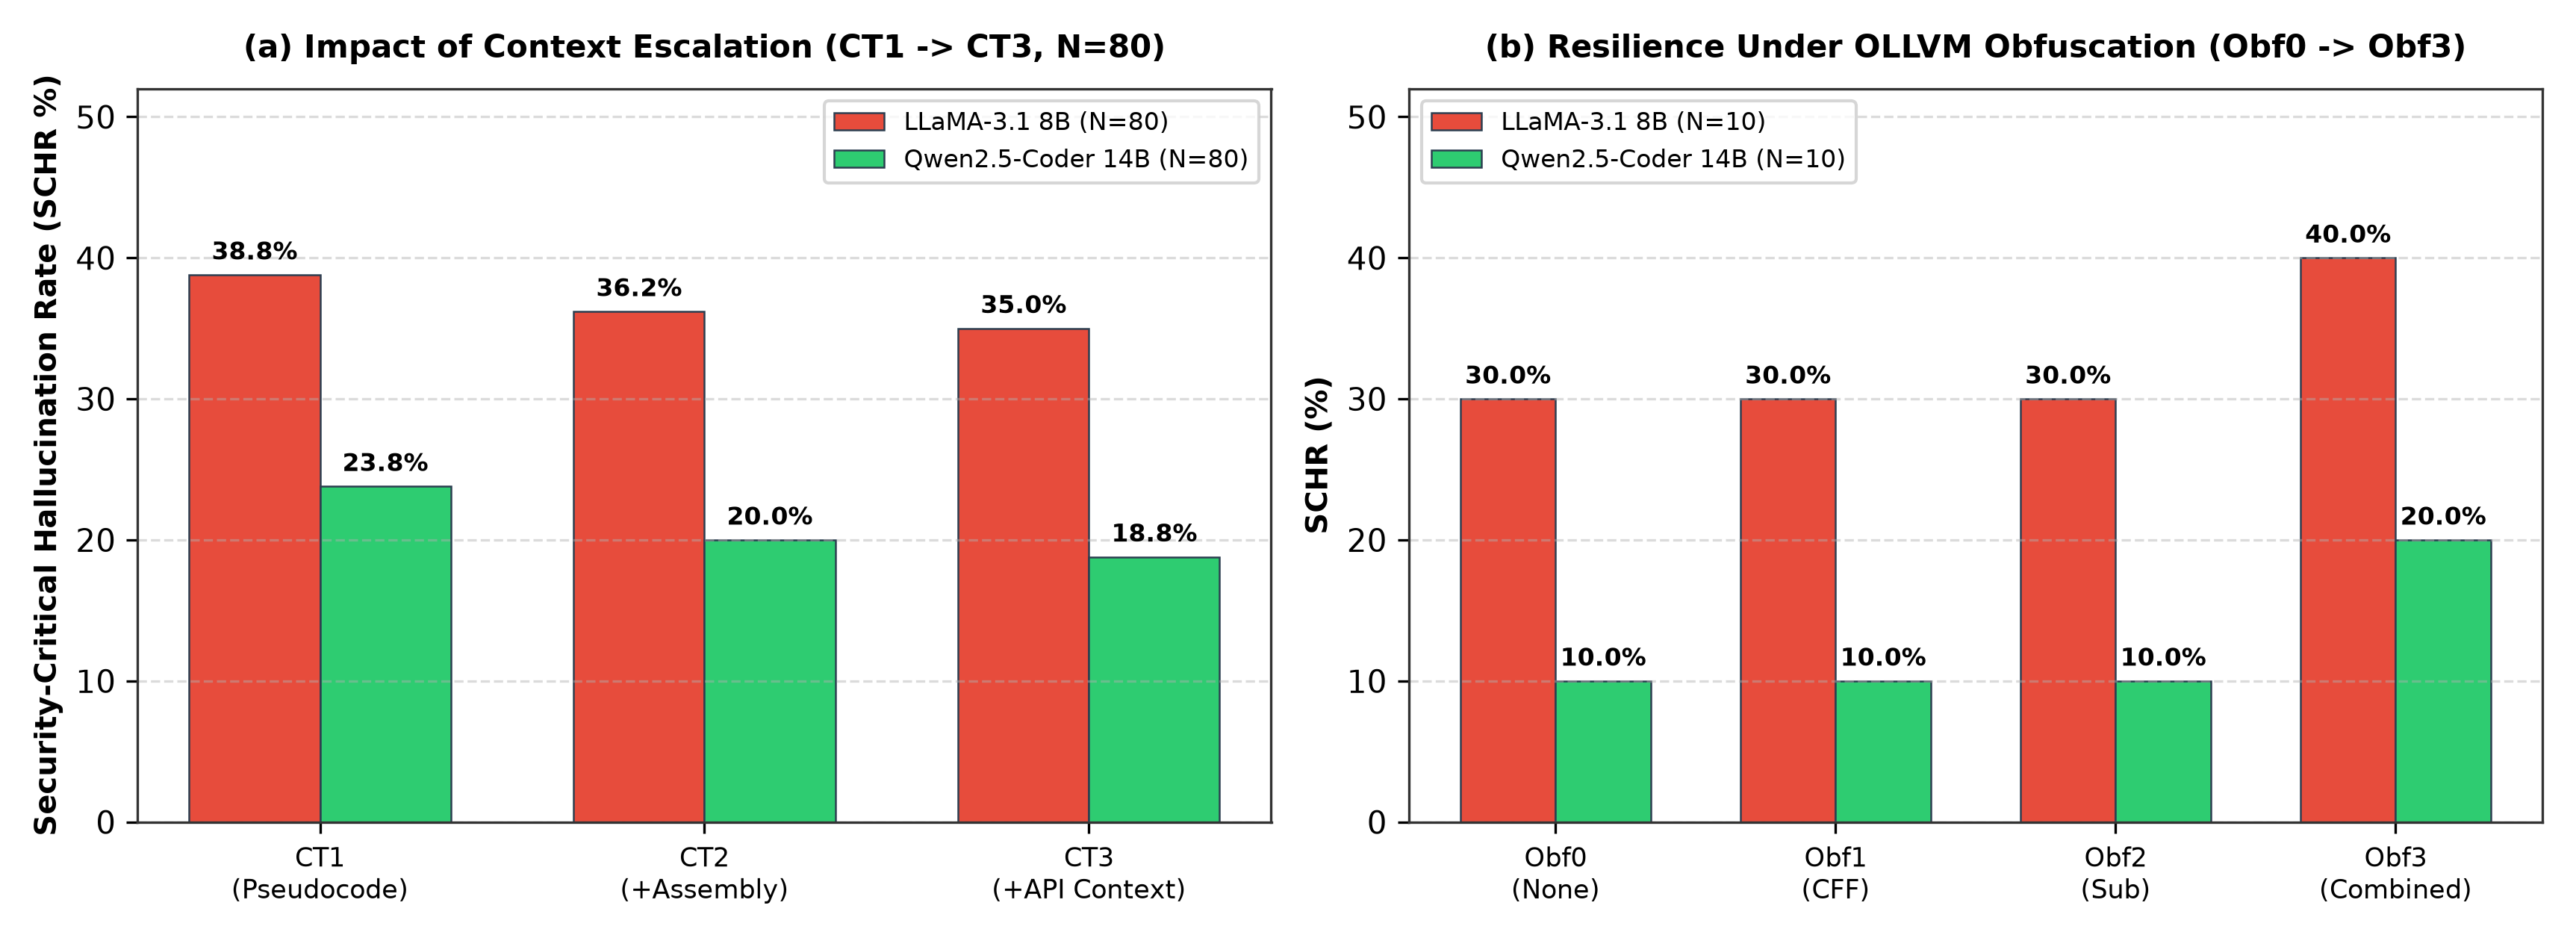
\includegraphics[width=\columnwidth]{figures/fig3_empirical_schr.png}
\caption{Visualizing SCHR trends across Context Escalation Tiers ($N=80$) and OLLVM Obfuscation configurations (\texttt{Obf0}--\texttt{Obf3}, $N=10$ stratified subset).}
\label{fig:empirical_schr}
\end{figure}

\section{Quantitative Evaluation and Empirical Findings}

\subsection{RQ1: Baseline Hallucination Rates Across Full Dataset ($N=80$)}
Table~\ref{tab:core_results} presents the empirical results across all 80 binaries (480 core evaluation runs logged in \path{results/benchmark_raw_logs.json}). Under standard decompiled pseudocode (CT1), the general-purpose \path{llama3.1:8b} model exhibits a baseline SCHR of \textbf{38.8\%} (31/80 errors, 95\% Wilson CI: [28.8\%, 49.7\%]) and a Mutant Miss Rate of \textbf{32.5\%} (13/40 mutants misclassified). In contrast, the code-specialized \path{qwen2.5-coder:14b} model achieves a significantly lower baseline CT1 SCHR of \textbf{23.8\%} (19/80 errors, 95\% Wilson CI: [15.8\%, 34.1\%]) and a Mutant Miss Rate of \textbf{27.5\%} (11/40), confirming that code-focused pretraining improves structural comprehension of stripped pseudocode, though at a $3.8\times$ higher mean inference latency (26.69s vs.\ 6.93s).

\begin{table*}[t]
\centering
\caption{Core Quantitative Evaluation across Context Tiers (CT1--CT3) on the complete 80-binary dataset ($N=80$ per tier, 480 runs total): SCHR (\%), 95\% Wilson CI, Mutant Miss Rate (\%), Pairwise BLEU-4 (Orig vs.\ Mut), and Mean Latency.}
\label{tab:core_results}
\footnotesize
\setlength{\tabcolsep}{5pt}
\begin{tabular}{@{}llcccccc@{}}
\toprule
\textbf{Model} & \textbf{Context Tier} & \textbf{Samples ($N$)} & \textbf{Hallucinations} & \textbf{SCHR (\%) [95\% Wilson CI]} & \textbf{Mutant Miss Rate (\%)} & \textbf{BLEU-4 (Orig vs.\ Mut)} & \textbf{Mean Latency (s)} \\
\midrule
\texttt{llama3.1:8b}       & \textbf{CT1 (Pseudocode)}  & 80 & 31 & \textbf{38.8\%} [28.8\%, 49.7\%] & 32.5\% (13/40) & 0.376 & 6.93s \\
\texttt{llama3.1:8b}       & \textbf{CT2 (+Assembly)}    & 80 & 29 & \textbf{36.2\%} [26.6\%, 47.2\%] & 27.5\% (11/40) & 0.400 & 7.33s \\
\texttt{llama3.1:8b}       & \textbf{CT3 (+API Context)} & 80 & 28 & \textbf{35.0\%} [25.5\%, 45.9\%] & 27.5\% (11/40) & 0.462 & 7.53s \\
\midrule
\texttt{qwen2.5-coder:14b} & \textbf{CT1 (Pseudocode)}  & 80 & 19 & \textbf{23.8\%} [15.8\%, 34.1\%] & 27.5\% (11/40) & 0.358 & 26.69s \\
\texttt{qwen2.5-coder:14b} & \textbf{CT2 (+Assembly)}    & 80 & 16 & \textbf{20.0\%} [12.7\%, 30.0\%] & 25.0\% (10/40) & 0.403 & 26.77s \\
\texttt{qwen2.5-coder:14b} & \textbf{CT3 (+API Context)} & 80 & 15 & \textbf{18.8\%} [11.7\%, 28.7\%] & 25.0\% (10/40) & 0.409 & 26.31s \\
\bottomrule
\end{tabular}
\end{table*}

Tables~\ref{tab:category_matrix} and \ref{tab:central_matrix} break down SCHR across the five functional categories ($n=16$ binaries per category) and five mutation operator families ($N=80$). Three key findings emerge:
\begin{enumerate}
    \item \textbf{Vulnerability on Bitwise/Arithmetic Decoders (Category S \& $\mathcal{M}_2$):} Both models struggle on Category S (Toy Byte Decoders), with \path{llama3.1:8b} reaching 56.2\%--62.5\% SCHR and \path{qwen2.5-coder:14b} remaining at 56.2\% (9/16) across all three tiers. Under $\mathcal{M}_2$ (Constant \& Arithmetic Alteration), both models exhibit a 50.0\% (12/24) error rate at CT1.
    \item \textbf{Superior Branch Tracking in Code-Specialized Models:} In Category A (Debug Policy) and Category E (Env Signal), \path{qwen2.5-coder:14b} reduces CT2/CT3 SCHR to 6.2\% (1/16) and 18.8\% (3/16) respectively, compared to 31.2\% (5/16) and 43.8\%--50.0\% for \path{llama3.1:8b}. In Category P (Persistence Mock), adding assembly context (CT2/CT3) eliminates errors in \path{qwen2.5-coder:14b} ($12.5\% \rightarrow \mathbf{0.0\%}$).
    \item \textbf{Condition Inversion ($\mathcal{M}_1$) vs.\ Relational Boundaries ($\mathcal{M}_4$):} At CT1, \path{llama3.1:8b} fails on 50.0\% (12/24) of $\mathcal{M}_1$ and 31.2\% (5/16) of $\mathcal{M}_4$, whereas \path{qwen2.5-coder:14b} achieves 20.8\% (5/24) on $\mathcal{M}_1$ and 6.2\% (1/16) on $\mathcal{M}_4$.
\end{enumerate}

\begin{table}[t]
\centering
\caption{Domain-Specific SCHR (\%) Breakdown across Categories A, S, P, E, C ($n=16$ binaries per category, $N=80$).}
\label{tab:category_matrix}
\scriptsize
\setlength{\tabcolsep}{2.2pt}
\begin{tabular}{@{}llccccc@{}}
\toprule
\textbf{Model} & \textbf{Tier} & \textbf{A: Debug} & \textbf{S: Decoder} & \textbf{P: Persist} & \textbf{E: Env} & \textbf{C: Flow} \\
\midrule
\texttt{llama3.1} & \textbf{CT1} & 43.8\% (7/16) & 56.2\% (9/16)  & 12.5\% (2/16) & 43.8\% (7/16) & 37.5\% (6/16) \\
\texttt{llama3.1} & \textbf{CT2} & 31.2\% (5/16) & 62.5\% (10/16) & 6.2\% (1/16)  & 50.0\% (8/16) & 31.2\% (5/16) \\
\texttt{llama3.1} & \textbf{CT3} & 31.2\% (5/16) & 62.5\% (10/16) & 6.2\% (1/16)  & 43.8\% (7/16) & 31.2\% (5/16) \\
\midrule
\texttt{qwen2.5}  & \textbf{CT1} & 12.5\% (2/16) & 56.2\% (9/16)  & 12.5\% (2/16) & 18.8\% (3/16) & 18.8\% (3/16) \\
\texttt{qwen2.5}  & \textbf{CT2} & 6.2\% (1/16)  & 56.2\% (9/16)  & \textbf{0.0\% (0/16)} & 18.8\% (3/16) & 18.8\% (3/16) \\
\texttt{qwen2.5}  & \textbf{CT3} & 6.2\% (1/16)  & 56.2\% (9/16)  & \textbf{0.0\% (0/16)} & 18.8\% (3/16) & 12.5\% (2/16) \\
\bottomrule
\end{tabular}
\end{table}

\begin{table}[t]
\centering
\caption{Central Matrix (E1--E3): SCHR (\%) across Mutation Operator Families ($\mathcal{M}_1$--$\mathcal{M}_5$, $N=80$).}
\label{tab:central_matrix}
\scriptsize
\setlength{\tabcolsep}{2.2pt}
\begin{tabular}{@{}llcccccc@{}}
\toprule
\textbf{Model} & \textbf{Tier} & \textbf{$\mathcal{M}_1$ (24)} & \textbf{$\mathcal{M}_2$ (24)} & \textbf{$\mathcal{M}_3$ (10)} & \textbf{$\mathcal{M}_4$ (16)} & \textbf{$\mathcal{M}_5$ (6)} & \textbf{Total} \\
\midrule
\texttt{llama3.1} & \textbf{CT1} & 50.0\% (12) & 50.0\% (12) & 10.0\% (1) & 31.2\% (5) & 16.7\% (1) & \textbf{38.8\%} \\
\texttt{llama3.1} & \textbf{CT2} & 33.3\% (8)  & 54.2\% (13) & 10.0\% (1) & 31.2\% (5) & 33.3\% (2) & \textbf{36.2\%} \\
\texttt{llama3.1} & \textbf{CT3} & 33.3\% (8)  & 54.2\% (13) & 0.0\% (0)  & 31.2\% (5) & 33.3\% (2) & \textbf{35.0\%} \\
\midrule
\texttt{qwen2.5}  & \textbf{CT1} & 20.8\% (5)  & 50.0\% (12) & 10.0\% (1) & 6.2\% (1)  & 0.0\% (0)  & \textbf{23.8\%} \\
\texttt{qwen2.5}  & \textbf{CT2} & 12.5\% (3)  & 45.8\% (11) & 0.0\% (0)  & 12.5\% (2) & 0.0\% (0)  & \textbf{20.0\%} \\
\texttt{qwen2.5}  & \textbf{CT3} & 12.5\% (3)  & 41.7\% (10) & 0.0\% (0)  & 12.5\% (2) & 0.0\% (0)  & \textbf{18.8\%} \\
\bottomrule
\end{tabular}
\end{table}

\subsection{RQ2: Disparity Between SCHR and Lexical Similarity (BLEU-4)}
As shown in Table~\ref{tab:core_results}, the pairwise BLEU-4 score between natural language explanations generated for original binaries ($\mathcal{Y}_{\text{orig}}$) and their mutated counterparts ($\mathcal{Y}_{\text{mut}}$) ranges from \textbf{0.376 to 0.462} for \path{llama3.1:8b} and \textbf{0.358 to 0.409} for \path{qwen2.5-coder:14b}. As context escalates from CT1 to CT3 on \path{llama3.1:8b}, pairwise lexical similarity increases from 0.376 to 0.462 even though the model continues to hallucinate on 35.0\% (28/80) of the binaries. Because flipping a conditional jump (\texttt{JZ} $\leftrightarrow$ \texttt{JNZ}) or altering a single constant leaves over 90\% of the surrounding function template unchanged, LLMs generate nearly identical textual descriptions for both variants while missing the inverted security outcome.

\subsection{RQ3: Context Escalation and McNemar's Paired Analysis}
Appending x86-64 disassembly (CT2) and API context (CT3) reduces point-estimate hallucination rates for both models: \path{llama3.1:8b} improves from 38.8\% $\rightarrow$ 36.2\% $\rightarrow$ 35.0\%, while \path{qwen2.5-coder:14b} improves from 23.8\% $\rightarrow$ 20.0\% $\rightarrow$ 18.8\%. Table~\ref{tab:mcnemar} reports McNemar's paired test across all 80 binaries. While adding assembly/API context rescues $b=6\text{--}8$ binaries in \path{llama3.1:8b} and $b=5\text{--}6$ binaries in \path{qwen2.5-coder:14b}, it simultaneously induces $c=4\text{--}5$ new errors in \path{llama3.1:8b} and $c=2$ new errors in \path{qwen2.5-coder:14b} ($p \in [0.2888, 0.7518]$) due to \textit{context dilution} and \textit{pseudocode primacy}.

\begin{table}[t]
\centering
\caption{McNemar's Paired Test comparing CT1 vs.\ CT2/CT3 ($N=80$). $b$: CT1 Err $\rightarrow$ Fix; $c$: CT1 Ok $\rightarrow$ Err.}
\label{tab:mcnemar}
\scriptsize
\setlength{\tabcolsep}{3pt}
\begin{tabular}{@{}llccccc@{}}
\toprule
\textbf{Model} & \textbf{Comparison} & \textbf{$b$ ($1\rightarrow 0$)} & \textbf{$c$ ($0\rightarrow 1$)} & \textbf{Net Gain} & \textbf{$\chi^2$} & \textbf{$p$-value} \\
\midrule
\texttt{llama3.1:8b}       & \textbf{CT1 vs.\ CT2} & 6 & 4 & $+2$ & 0.100 & 0.7518 \\
\texttt{llama3.1:8b}       & \textbf{CT1 vs.\ CT3} & 8 & 5 & $+3$ & 0.308 & 0.5791 \\
\midrule
\texttt{qwen2.5-coder:14b} & \textbf{CT1 vs.\ CT2} & 5 & 2 & $+3$ & 0.571 & 0.4497 \\
\texttt{qwen2.5-coder:14b} & \textbf{CT1 vs.\ CT3} & 6 & 2 & $+4$ & 1.125 & 0.2888 \\
\bottomrule
\end{tabular}
\end{table}

\subsection{RQ4: Resilience Under Binary Obfuscation}
\label{sec:rq4}
To evaluate adversarial resilience (Experiment E4), we benchmarked both models across four OLLVM levels (\texttt{Obf0}, \path{Obf1_CFF}, \path{Obf2_Sub}, and \path{Obf3_Combined}) on a stratified 10-binary subsample (60 obfuscation runs logged in \path{benchmark_raw_logs.json}). As shown in Table~\ref{tab:obfuscation}, isolated \path{Obf1_CFF} or \path{Obf2_Sub} maintains baseline error rates (30.0\% for LLaMA-3.1; 10.0\% for Qwen2.5-Coder), whereas combined protection (\path{Obf3_Combined}) pushes \path{llama3.1:8b} SCHR to \textbf{40.0\%} [16.8\%, 68.7\%] and doubles \path{qwen2.5-coder:14b} SCHR from 10.0\% to \textbf{20.0\%} [5.7\%, 51.0\%].

\begin{table}[t]
\centering
\caption{Effect of OLLVM Obfuscation Levels (\texttt{Obf0}--\texttt{Obf3}) on SCHR (\%) ($N=10$ stratified subset).}
\label{tab:obfuscation}
\scriptsize
\setlength{\tabcolsep}{2.8pt}
\begin{tabular}{@{}llccc@{}}
\toprule
\textbf{Model} & \textbf{Obfuscation Level} & \textbf{Samples} & \textbf{Errors} & \textbf{SCHR [95\% Wilson CI]} \\
\midrule
\texttt{llama3.1:8b}   & Obf0 (Unobfuscated) & 10 & 3 & 30.0\% [10.8\%, 60.3\%] \\
\texttt{llama3.1:8b}   & Obf1\_CFF (Flattening) & 10 & 3 & 30.0\% [10.8\%, 60.3\%] \\
\texttt{llama3.1:8b}   & Obf2\_Sub (Substitution) & 10 & 3 & 30.0\% [10.8\%, 60.3\%] \\
\texttt{llama3.1:8b}   & Obf3\_Combined & 10 & 4 & \textbf{40.0\%} [16.8\%, 68.7\%] \\
\midrule
\texttt{qwen2.5-coder} & Obf0 (Unobfuscated) & 10 & 1 & 10.0\% [1.8\%, 40.4\%] \\
\texttt{qwen2.5-coder} & Obf1\_CFF (Flattening) & 10 & 1 & 10.0\% [1.8\%, 40.4\%] \\
\texttt{qwen2.5-coder} & Obf2\_Sub (Substitution) & 10 & 1 & 10.0\% [1.8\%, 40.4\%] \\
\texttt{qwen2.5-coder} & Obf3\_Combined & 10 & 2 & \textbf{20.0\%} [5.7\%, 51.0\%] \\
\bottomrule
\end{tabular}
\end{table}

\subsection{Comparative Analysis Against Prior Benchmarks}
Table~\ref{tab:sota_comparison} compares SCHR-Bench with prior decompilation benchmarks (VeRA~\cite{alrabaee2022vera}, Decompile-Eval~\cite{decompileeval2024}, LLM4Decompile~\cite{sun2024llm4decompile}, and RevLLM~\cite{revllm2024}).

\begin{table*}[t]
\centering
\caption{Comparative Analysis: SCHR-Bench versus Existing Decompilation and SRE Benchmarks.}
\label{tab:sota_comparison}
\scriptsize
\setlength{\tabcolsep}{4pt}
\begin{tabular}{@{}lcccccc@{}}
\toprule
\textbf{Benchmark Framework} & \textbf{Target Domain} & \textbf{Ground Truth Foundation} & \textbf{Evaluated Metric} & \textbf{Obfuscation Support} & \textbf{Malware Case Study} & \textbf{Deterministic Security Oracle} \\
\midrule
VeRA (IEEE S\&P '22)~\cite{alrabaee2022vera} & Variable \& Type RE & Source Symbol Tables & TypeAcc / Identifiers & None & None & Symbol Table Overlap (Non-executable) \\
Decompile-Eval (ACL '24)~\cite{decompileeval2024} & Algorithm Syntax & LeetCode Unit Tests & Re-executability & None & None & Unit Tests (Syntax Pass Rate) \\
LLM4Decompile (EMNLP '24)~\cite{sun2024llm4decompile} & Neural Decompilation & C Source Code & BLEU-4 & None & None & Lexical BLEU-4 Only \\
RevLLM (2024)~\cite{revllm2024} & SRE Intent & Human Annotations & Qualitative Overlap & Light (Symbolic) & Snippets & Manual Heuristic Tags \\
\midrule
\textbf{SCHR-Bench (Ours)} & \textbf{Security-Critical SRE} & \textbf{Binary Mutation Invariants} & \textbf{SCHR (\%) [Wilson 95\% CI]} & \textbf{OLLVM Obf0--Obf3} & \textbf{Gh0stRAT PE32} & \textbf{160 Dynamic Assertions (E0)} \\
 & \textbf{(Categories A, S, P, E, C)} & \textbf{($N=80$ Binaries, 540 Runs)} & \textbf{\& Mutant Miss Rate} & \textbf{(+10.0 pp under Obf3)} & \textbf{(Static Triage)} & \textbf{(100\% Behavioral Divergence)} \\
\bottomrule
\end{tabular}
\end{table*}

\section{Error Taxonomy and Static Malware Case Study}

\subsection{Empirical Hallucination Taxonomy Across CT1 ($N=50$ Error Events)}
Across the 160 CT1 evaluations (80 binaries $\times$ 2 models), \textbf{50 SCHR hallucination events} occurred (31 from \path{llama3.1:8b} and 19 from \path{qwen2.5-coder:14b}). Table~\ref{tab:error_taxonomy} classifies all 50 logged CT1 failures by their underlying mutation mechanism in \path{benchmark_raw_logs.json}: Constant \& Arithmetic Corruption accounts for 48.0\% (24/50), Branch \& Boolean Polarity Inversion accounts for 34.0\% (17/50), Relational Boundary Shift accounts for 12.0\% (6/50), and Target Swap / Step Omission accounts for 6.0\% (3/50).

\begin{table}[t]
\centering
\caption{Empirical Hallucination Taxonomy across all 50 logged CT1 failure events in \texttt{results/benchmark\_raw\_logs.json}.}
\label{tab:error_taxonomy}
\scriptsize
\setlength{\tabcolsep}{3.5pt}
\begin{tabular}{@{}lccc@{}}
\toprule
\textbf{Failure Mode Category} & \textbf{LLaMA ($n=31$)} & \textbf{Qwen ($n=19$)} & \textbf{Total ($N=50$)} \\
\midrule
\textbf{Constant \& Arithmetic Corruption} & 12 & 12 & \textbf{24 (48.0\%)} \\
\textbf{Branch \& Boolean Inversion}       & 12 & 5  & \textbf{17 (34.0\%)} \\
\textbf{Relational Boundary Shift}         & 5  & 1  & \textbf{6 (12.0\%)}  \\
\textbf{Target Swap \& Step Omission}      & 2  & 1  & \textbf{3 (6.0\%)}   \\
\bottomrule
\end{tabular}
\end{table}

\subsection{Static Triage Case Study: In-the-Wild Gh0stRAT PE32}
To bridge our controlled benchmark with real-world malware triage, we conducted a strictly static inspection on an in-the-wild \textbf{Gh0stRAT} PE32 binary (SHA-256 prefix: \path{ea7cd59c402128b0...62cb4aa51e605d3bcaee98be}~\cite{mitre2024gh0st,malwarebazaar_gh0st}) inside Tier 3 using DIE v3.21 and PE-bear v0.7.2, with \textbf{zero runtime execution}.

Static triage revealed that the binary is protected by \textbf{VXiProtect / VMProtect (v3.6.0+)}: section \texttt{.O\#J} exhibits a packed entropy of \textbf{7.89 bits/byte}, the IAT exposes only dynamic resolver stubs (\path{LoadLibraryA}, \path{GetProcAddress}), and raw static string searches for \path{Software\Microsoft\Windows\CurrentVersion\Run} return \textbf{0 matches} (\path{tier3_win11/Image_Result/}). While an unanchored LLM asked to inspect raw packed PE headers hallucinates fabricated IAT imports, evaluating representative decompiled unpacker-stub (\path{CS01_GH0STRAT_PACKER_ENTRY}) and registry-persistence (\path{CS02_GH0STRAT_PERSISTENCE_INSTALL}) routines in \path{results/GH0STRAT_EVALUATION.json} shows that both \path{llama3.1:8b} (confidence 0.90) and \path{qwen2.5-coder:14b} (confidence 0.95) accurately classify the explicit \path{GetProcAddress} + \texttt{0xA7} XOR loop and \path{RegSetValueExA} routine as malicious under CT1 and CT2. This contrast reinforces our core thesis: LLMs reliably recognize canonical high-level API patterns when visible, but fail when commercial packing hides the IAT or when subtle logic mutations ($\mathcal{M}_1, \mathcal{M}_2$) alter underlying semantics without changing surface syntax.

\section{Discussion, Threats to Validity, and Conclusion}

\subsection{Mitigating Pseudocode Primacy and Threats to Validity}
Our McNemar analysis ($p \in [0.2888, 0.7518]$) demonstrates that simply appending disassembly onto pseudocode yields modest net gains ($+2$ to $+4$ binaries) because models suffer from \textit{pseudocode primacy} and \textit{context dilution}. Future SRE copilot architectures should enforce \textbf{Interleaved Chain-of-Thought (CoT) Alignment}---requiring models to map each pseudocode predicate to its exact assembly instruction (\texttt{CMP}/\texttt{JNZ}) before predicting outcomes---and \textbf{Multi-Engine MCP Consensus} across Ghidra and Binary Ninja.

\textbf{Threats to Validity:} (1) \textit{Construct Validity:} Our 40 C function pairs use controlled local security-logic kernels (\texttt{int target(int a, int b, int c)}) rather than live OS API calls to guarantee deterministic E0 execution and safety; while this abstracts away OS state, it isolates pure control-flow and arithmetic reasoning where decompiler hallucinations originate. (2) \textit{Statistical Power on E4:} While E1--E3 evaluate all $N=80$ binaries (480 runs), E4 evaluates a stratified $N=10$ subsample (60 runs); expanding OLLVM evaluation to all 80 binaries and 32B+ models is immediate future work.

\subsection{Conclusion and Reproducibility}
We presented \textbf{SCHR-Bench}, an execution-verified benchmark quantifying security-critical hallucinations in LLM-assisted binary reverse engineering across 80 stripped binaries and 540 logged runs. Our findings prove that surface lexical similarity ($\text{BLEU-4} \approx 0.36\text{--}0.46$) masks severe semantic errors (38.8\% CT1 SCHR on LLaMA-3.1 8B; 23.8\% on Qwen2.5-Coder 14B), bitwise decoders remain highly error-prone (56.2\% SCHR), and combined OLLVM obfuscation elevates hallucinations up to 40.0\%. All C sources, compiled binaries, Ghidra scripts, and raw JSON logs are publicly accessible at \url{https://github.com/phat1310/IAM302t_SCHR_Bench}.

\balance
\bibliographystyle{IEEEtran}
\bibliography{references}

\end{document}
